\documentclass{article}
\usepackage{kotex}
\usepackage{setspace}
\usepackage[pdftex]{color, graphicx}
\usepackage[left=2.5cm,right=2.5cm,top=3cm,bottom=3cm,a4paper]{geometry}
\begin{document}
	\doublespacing
	\noindent 이번에는 표와 그림에 대해서 봅시다.\\
	먼저 표는 이렇게 그리면 됩니다.
	\begin{table}[hp]
		\centering
		\begin{tabular}{|c|c|}
			\hline
			그냥 & 이런\\
			\hline
			식으로 & 하면\\
			\hline
			표가 & 됩니다\\
			\hline
		\end{tabular}
	\caption{캡션은 이렇게 답니다}
	\label{tab:eg}
	\end{table}
	참 쉽죠?\\
	다음은 그림입니다.
	\begin{figure}[hp]
		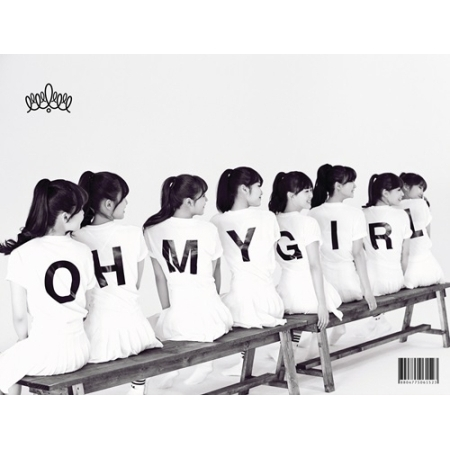
\includegraphics[width=0.9\textwidth]{OhMyGirl.jpg}
		\caption{그림도 캡션이 됩니다}
		\label{fig:eg}
	\end{figure}
\end{document}